% !TeX spellcheck = en_GB
\ifcsname SlidesDistr\endcsname%
	\documentclass[handout,aspectratio=169]{beamer}
\else%
	\documentclass[aspectratio=169]{beamer}
\fi%
\usepackage{fontspec}
\usepackage[T1]{fontenc}
\usepackage{amsmath}
\usepackage{amsfonts}
\usepackage{amssymb}
\usepackage{graphicx}
\usepackage{csquotes}
\usepackage{booktabs}
\usepackage{multicol}
\usepackage{enumerate}
\usepackage{microtype}
\usepackage[labelfont=bf,font={small}]{caption}
\usepackage{hyperref}
\usepackage{booktabs}
\usepackage{subcaption}
\usepackage{fancyhdr}
\usepackage{pdfpages}
\usepackage{siunitx}
\usepackage{tikz}
\usepackage{mdframed}

\defaultfontfeatures{Mapping=tex-text}
\newfontfamily\symbolfont{Symbola}
\newfontfamily\quotefont{Gentium}

\usepackage[sorting=none]{biblatex}
\addbibresource{../bibliography.bib}

\author{Andreas Stöckel}


\renewcommand{\vec}[1]{{\mathbf{#1}}}
\newcommand{\mat}[1]{{\mathbf{#1}}}
\newcommand{\T}{\ensuremath{\mathsf{T}}}
\renewcommand{\epsilon}{\varepsilon}
\renewcommand{\phi}{\varphi}

% Tango color palette
\definecolor{butter1}{HTML}{FCE94F}
\definecolor{butter2}{HTML}{EDD400}
\definecolor{butter3}{HTML}{C4A000}
\definecolor{orange1}{HTML}{FCAF3E}
\definecolor{orange2}{HTML}{F57900}
\definecolor{orange3}{HTML}{CE5C00}
\definecolor{chocolate1}{HTML}{E9B96E}
\definecolor{chocolate2}{HTML}{C17D11}
\definecolor{chocolate3}{HTML}{8F5902}
\definecolor{chameleon1}{HTML}{8AE234}
\definecolor{chameleon2}{HTML}{73D216}
\definecolor{chameleon3}{HTML}{4E9A06}
\definecolor{skyblue1}{HTML}{729FCF}
\definecolor{skyblue2}{HTML}{3465A4}
\definecolor{skyblue3}{HTML}{204A87}
\definecolor{plum1}{HTML}{AD7FA8}
\definecolor{plum2}{HTML}{75507B}
\definecolor{plum3}{HTML}{5C3566}
\definecolor{scarletred1}{HTML}{EF2929}
\definecolor{scarletred2}{HTML}{CC0000}
\definecolor{scarletred3}{HTML}{A40000}
\definecolor{aluminium1}{HTML}{EEEEEC}
\definecolor{aluminium2}{HTML}{D3D7CF}
\definecolor{aluminium3}{HTML}{BABDB6}
\definecolor{aluminium4}{HTML}{888A85}
\definecolor{aluminium5}{HTML}{555753}
\definecolor{aluminium6}{HTML}{2E3436}

\definecolor{violet}{HTML}{AA305C}
\definecolor{uwyellow}{HTML}{FDD433}
\definecolor{background}{HTML}{F9F9F6}
\definecolor{text}{HTML}{000000}

\definecolor{uweng1}{HTML}{D1B2EE}
\definecolor{uweng2}{HTML}{BF33DE}
\definecolor{uweng3}{HTML}{8001B3}
\definecolor{uweng4}{HTML}{56048A}

\setbeamercolor{title}{fg=violet}
\setbeamercolor{frametitle}{fg=black}
\setbeamercolor{structure}{fg=aluminium5}
\setbeamercolor{normal text}{fg=text}

\setbeamertemplate{navigation symbols}{}
\setbeamertemplate{footline}[frame number]

\hypersetup{%
	colorlinks=false,% hyperlinks will be black
	urlbordercolor=aluminium4,% hyperlink borders will be red
	pdfborderstyle={/S/U/W 0.5}% border style will be underline of width 1pt
}

\makeatletter
\newcommand{\superimpose}[2]{%
	{\ooalign{{#1}\hidewidth\cr{#2}\hidewidth\cr}}}
\makeatother
\newcommand{\SolidCircle}[2]{\superimpose{\color{#1}\symbolfont ⬤}{\textbf{\color{white}#2}}\hspace{1em}}
\newcommand{\OPlus}{\SolidCircle{chameleon3}{\kern0.75pt+}}
\newcommand{\OMeh}{\SolidCircle{uwyellow}{~}}
\newcommand{\OMinus}{\SolidCircle{scarletred3}{\kern2.25pt--}}

\newcommand{\hl}[1]{\colorbox{uwyellow}{{\color{black}\textbf{#1}}}}

\newcommand{\ImageSources}[1]{%
	\begin{columns}%
		\column{1.1\textwidth}%
		\raggedright%
		\tiny\color{aluminium4}%
		\setlength\lineskip{1em}%
		\textbf{Image Sources.}	{#1}%
	\end{columns}}

\newcommand{\ColorRect}[3]{{\color{#1}\rule{#2}{#3}}}
\setbeamertemplate{headline}{\ColorRect{black}{\textwidth}{4pt}\newline\ColorRect{uweng1}{0.25\textwidth}{4pt}\ColorRect{uweng2}{0.25\textwidth}{4pt}\ColorRect{uweng3}{0.25\textwidth}{4pt}\ColorRect{uweng4}{0.25\textwidth}{4pt}}

\newcommand{\MakeTitle}{%
	\vspace{0.5cm}%
	{\textbf{\inserttitle}}\\[0.5cm]%
	\insertauthor\\[0.5cm]%
	\insertdate\\%
	\vspace{2cm}%
 	
\includegraphics[width=7cm]{../assets/uwlogo_eng.pdf}%
}

\newcommand{\handwritingframe}{%
	\begin{frame}
		\begin{columns}
			\column{\paperwidth}
			
\includegraphics{../assets/handwriting_lines.pdf}
		\end{columns}
	\end{frame}	
}

\newcommand{\imageframe}[1]{%
	\setbeamertemplate{navigation symbols}{}%
	\begin{frame}[plain,noframenumbering]%
		\begin{tikzpicture}[remember picture,overlay]%
		\node[at=(current page.center)] {%
			\includegraphics[width=\paperwidth]{#1}%
		};%
		\end{tikzpicture}%
	\end{frame}%
}

\newcommand{\videoframe}[3][mp4]{%
	\begin{frame}[plain,noframenumbering]%
		\hypersetup{%
			pdfborderstyle={/S/U/W 0}% border style will be underline of width 1pt
		}%
		\begin{tikzpicture}[remember picture,overlay]%
		\node[at=(current page.center)] {%
			\includegraphics[width=\paperwidth]{{{video/#2_#3}.jpg}}%
		};%
		\node[at=(current page.center)] {%
			\ifcsname SlidesDistr\endcsname%
				\href{https://youtu.be/#3}{
\includegraphics[width=2cm]{../assets/play_button.pdf}}%
			\else%
				\href{video/#2_#3.#1}{
\includegraphics[width=2cm]{../assets/play_button.pdf}}%
			\fi%
		};%
		\end{tikzpicture}%
	\end{frame}%
}

\newcommand{\includevideo}[4][mp4]{%
	\begingroup%
	\hypersetup{%
		pdfborderstyle={/S/U/W 0}% border style will be underline of width 1pt
	}%
	\begin{tikzpicture}%
	\node (A) {%
		\includegraphics[width=#4]{{{video/#2_#3}.jpg}}%
	};%
	\node[at=(A.center)] {%
		\ifcsname SlidesDistr\endcsname%
			\href{https://youtu.be/#3}{
\includegraphics[width=2cm]{../assets/play_button.pdf}}%
		\else%
			\href{video/#2_#3.#1}{
\includegraphics[width=2cm]{../assets/play_button.pdf}}%
		\fi%
	};%
	\end{tikzpicture}%
	\endgroup%
}

\newcommand{\backupbegin}{
	\newcounter{finalframe}
	\setcounter{finalframe}{\value{framenumber}}
	\setbeamertemplate{footline}{}
}

\newcommand{\backupend}{
	\setcounter{framenumber}{\value{finalframe}}
}


\date{September 13 \& 15, 2021}
\title{SYDE 556/750 \\ Simulating Neurobiological Systems \\ Lecture 3 and 4: Population Representation}

\begin{document}
	
\begin{frame}{}
	\vspace{0.5cm}
	\begin{columns}[c]
		\column{0.6\textwidth}
		\MakeTitle
		\column{0.4\textwidth}
		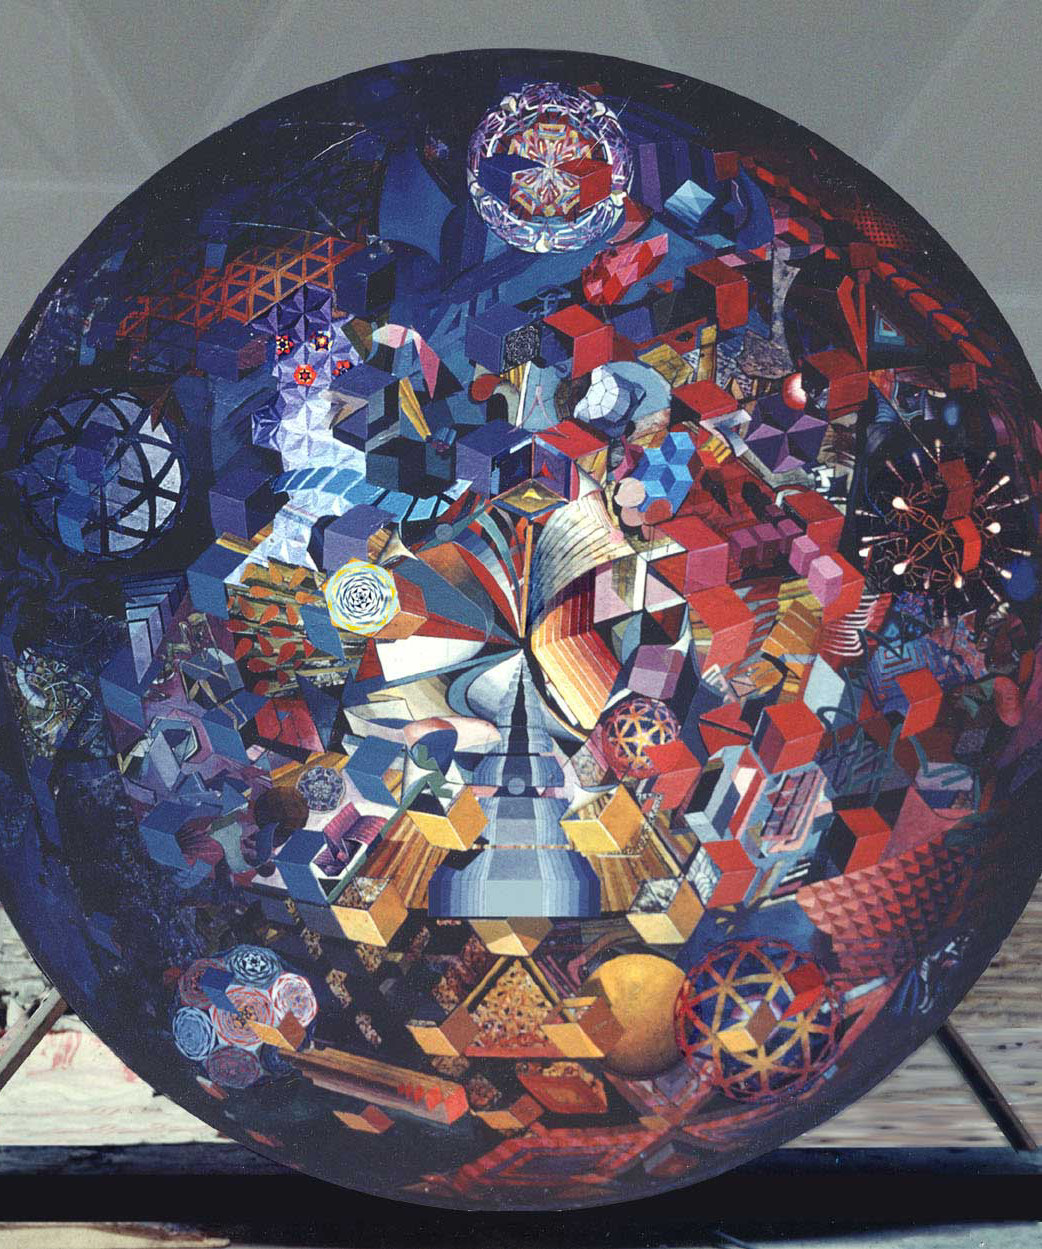
\includegraphics[width=\textwidth]{media/cubism_the_ultimate_painting_small.jpg}
	\end{columns}
\end{frame}

\videoframe[webm]{visual_cortex}{KE952yueVLA}

\videoframe[webm]{hippocampal_place_cells}{lfNVv0A8QvI}

\begin{frame}{NEF Principle 1: Representation}
	\begin{mdframed}
		\textbf{NEF Principle 1 -- Representation}\\
		\emph{Groups} (\enquote{populations}, or \enquote{ensembles}) of neurons \emph{represent} represent values via nonlinear encoding and linear decoding.
	\end{mdframed}
\end{frame}

\begin{frame}{Lossless Codes}
	\vspace{0.5cm}
	\begin{columns}
		\column{0.6\textwidth}
		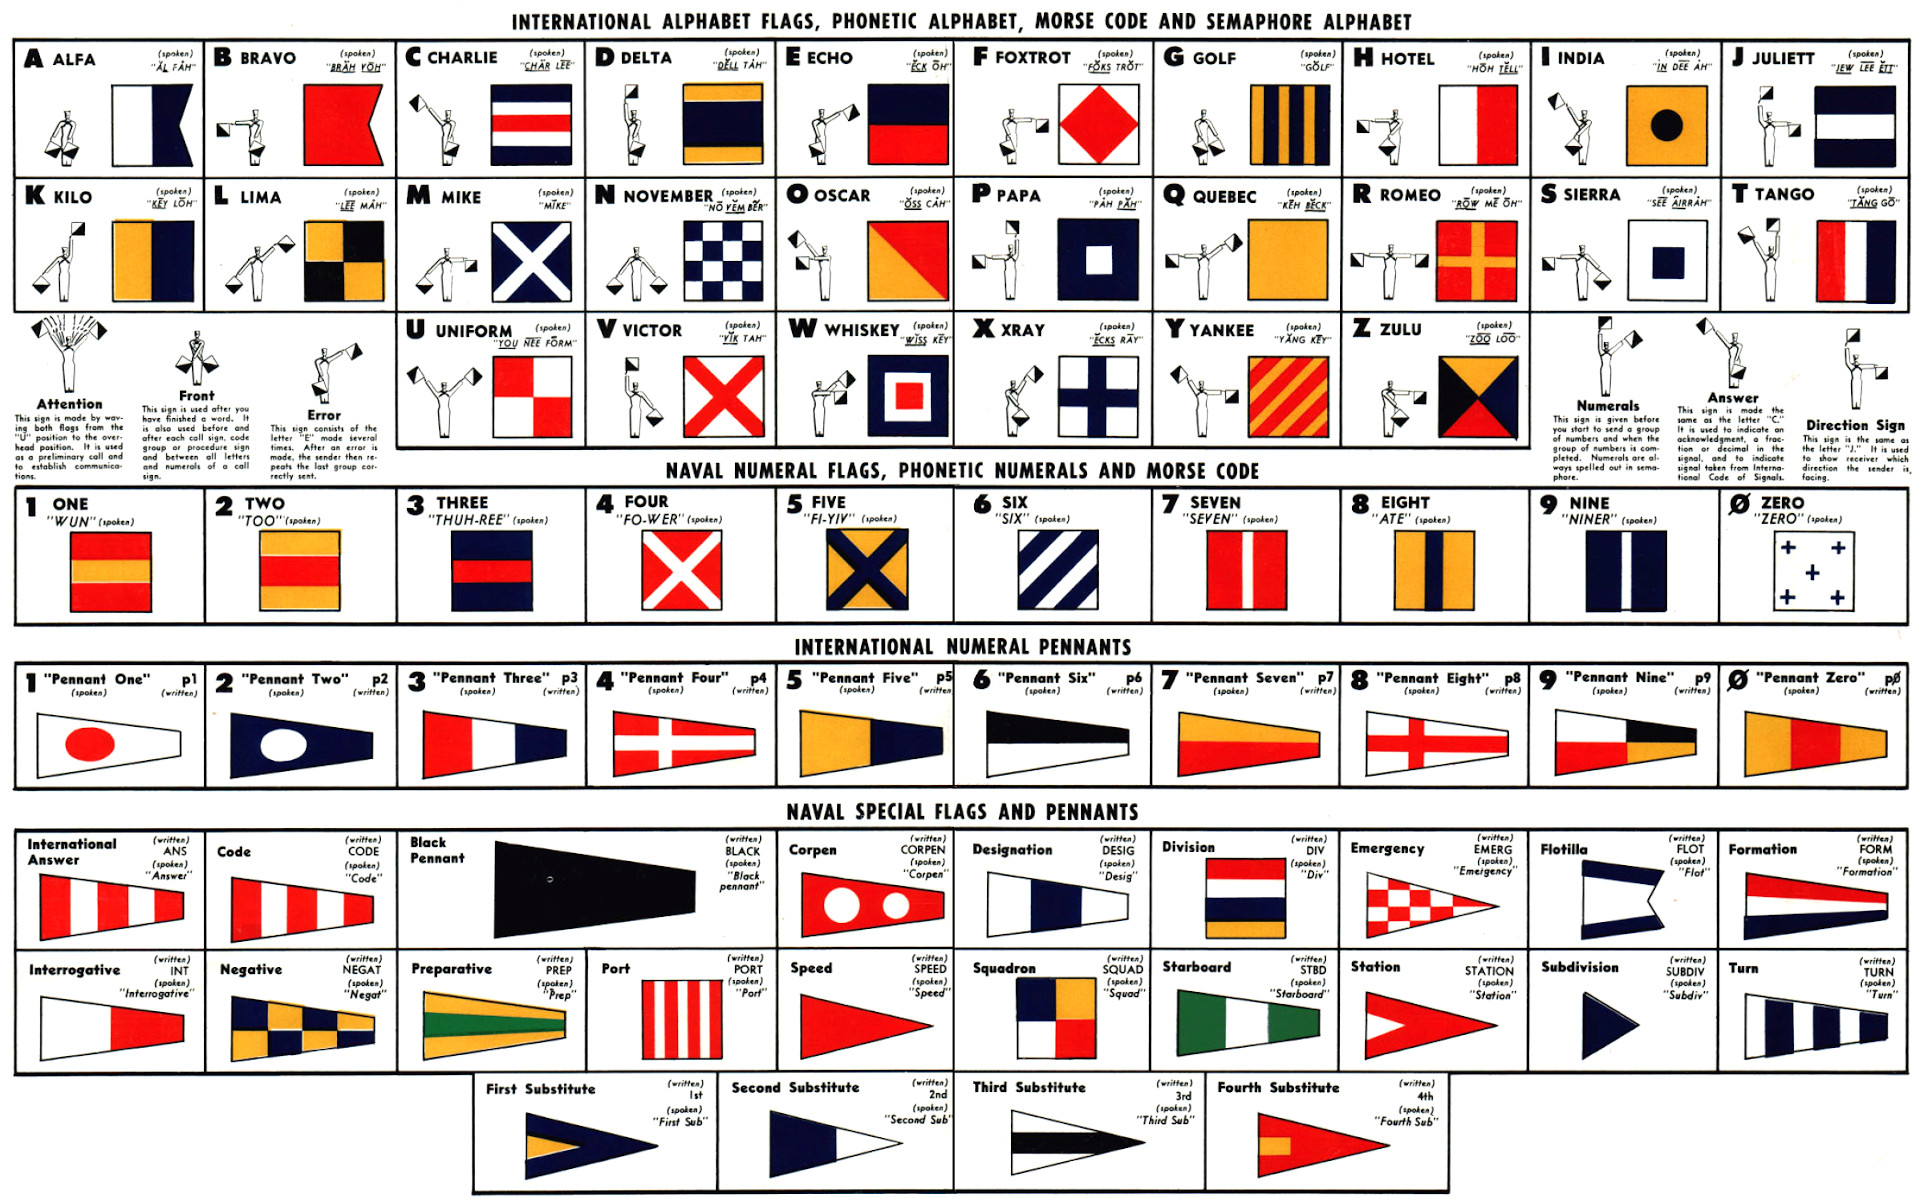
\includegraphics[width=\textwidth]{media/flag_alphabet_1956_small.jpg}
		\column{0.4\textwidth}
		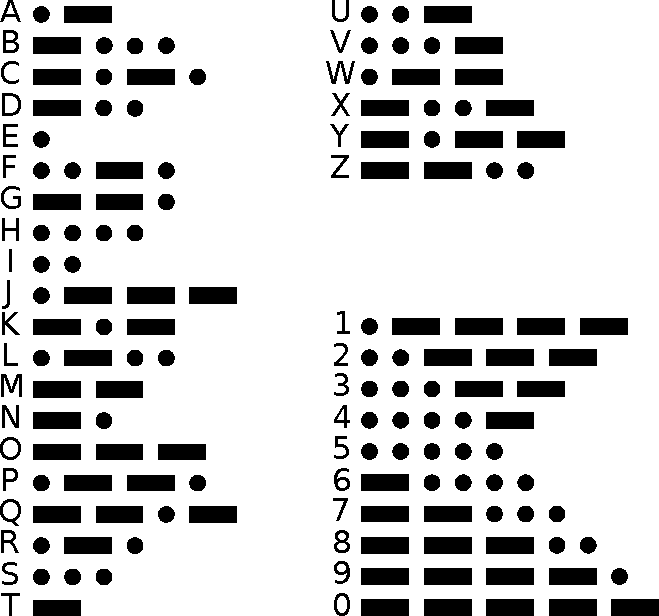
\includegraphics[width=\textwidth]{media/international_morse_code.pdf}
	\end{columns}
	\vspace{0.25cm}
	\begin{align*}
		\text{Encoding:} \quad \vec a &= f(\vec x) & \text{Decoding:} \quad \vec x &= f^{-1}(\vec a)
	\end{align*}
\end{frame}

\begin{frame}{Binary numbers: Nonlinear encoding, linear decoding}
	\begin{itemize}
		\setlength{\itemsep}{0.25cm}
		\item Represent a natural number between $0$ and $2^{n} - 1$ as $n$ binary digits.
		\item<2-> \textbf{Nonlinear encoding}
			\begin{align*}
			a_i &= \big(f(x)\big)_i = \begin{cases}
				1 & \text{if } x - 2^i \left\lfloor \frac{x}{2^i} \right\rfloor > 2^{i - 1} \,,\\
				0 & \text{otherwise} \,.
				\end{cases}
			\end{align*}
		\item<3-> \textbf{Linear decoding}\\[-1cm]
		\begin{align*}
			x &= f^{-1}(\vec a) = \sum_{i=0}^{n -1} 2^i a_i = \mat F \vec a = \begin{pmatrix} 1 & 2 & \ldots & 2^{n - 1}\end{pmatrix} \begin{pmatrix} a_0 \\ a_1 \\ \vdots \\ a_{n - 1} \end{pmatrix} \,.
		\end{align*}
		\item<4-> This is a \hl{distributed code}. \only<5->{But, \hl{not robust} against additive noise!}
	\end{itemize}
\end{frame}

\begin{frame}{Lossy codes}
	\begin{itemize}
		\setlength{\itemsep}{0.5cm}
		\item \textbf{Lossy code}\\
		Inverse $f^{-1}$ does not exist, instead \emph{approximate} the represented value
		\begin{align*}
			\text{Encoding:} \quad \vec a &= f(\vec x) & \text{Decoding:} \quad \vec x &\approx g(\vec a)
		\end{align*}
		\item<2-> \textbf{Examples}\\
		\begin{itemize}
			\setlength{\itemsep}{0.25cm}
			\item Audio, image, and video coding schemes\\(MP3, JPEG, H.264)\\
			\item Basis transformation onto first $n$ principal components (PCA)\\
			\item<3-> \textbf{Neural Representations}
		\end{itemize}
	\end{itemize}
\end{frame}

\begin{frame}{Tuning curves (I)}
	\begin{columns}
		\column{0.5\textwidth}
		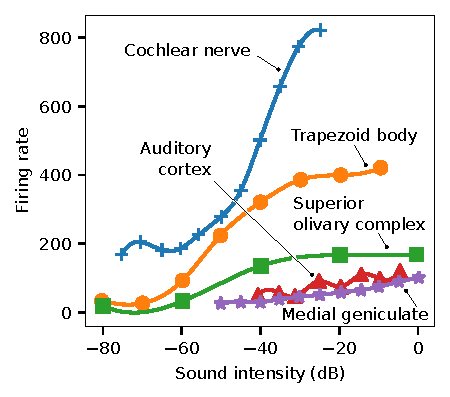
\includegraphics[width=\textwidth]{media/audition_tuning_curves_annotated.pdf}%
		\column{0.5\textwidth}
		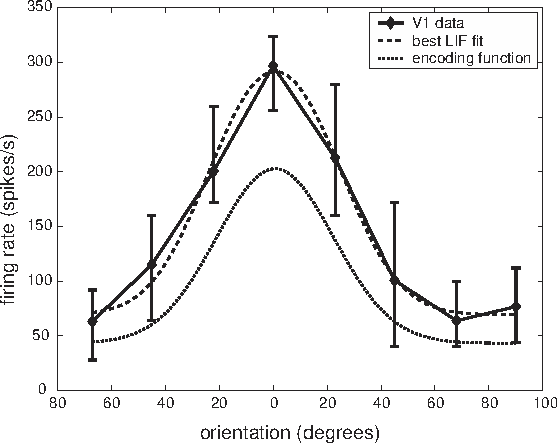
\includegraphics[width=\textwidth]{media/eliasmith_et_al_2003_orientation_tuning.pdf}%
	\end{columns}
\end{frame}

\begin{frame}{Tuning curves (II)}
	\begin{columns}
		\column{0.25\textwidth}
		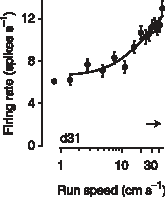
\includegraphics[scale=1.25]{media/saleem_et_al_tuning_curves_a.pdf}
		\column{0.25\textwidth}
		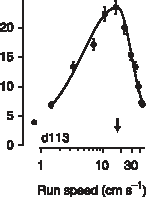
\includegraphics[scale=1.25]{media/saleem_et_al_tuning_curves_b.pdf}
		\column{0.25\textwidth}
		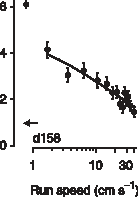
\includegraphics[scale=1.25]{media/saleem_et_al_tuning_curves_c.pdf}
		\column{0.25\textwidth}
		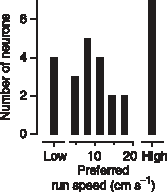
\includegraphics[scale=1.25]{media/saleem_et_al_tuning_curves_d.pdf}
	\end{columns}
\end{frame}



\begin{frame}
	\begin{columns}
		\column{0.5\textwidth}
		\begin{itemize}
			\item Last lecture: response curves: $a=G(J)$
			\item This lecture: tuning curves: $a=f(x) = G(J_i(x))$
			\item What sort of function can we try for $J_i(x)$?
			\item<2-> Introduce a gain $\alpha_i$ and a bias $J^\mathrm{bias}_i$:
			\begin{align*}
				J_i(x) &= \alpha_i x + J^\mathrm{bias}_i \\
				a_i(x) &= G(\alpha_i x + J^\mathrm{bias}_i)			
			\end{align*}
			\item<2-> $\alpha_i$ controls the slope
			\item<2-> $J^\mathrm{bias}_i$ shifts curve left and right		
		\end{itemize}
		\column{0.5\textwidth}
		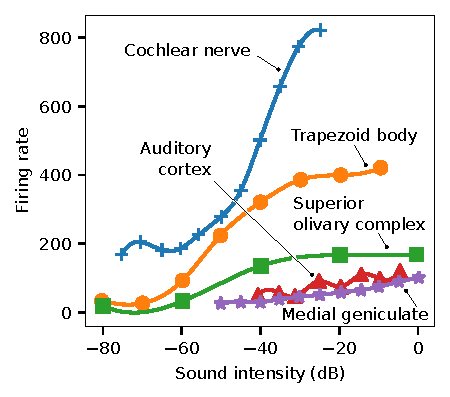
\includegraphics[width=0.7\textwidth]{media/audition_tuning_curves_annotated.pdf}\\
		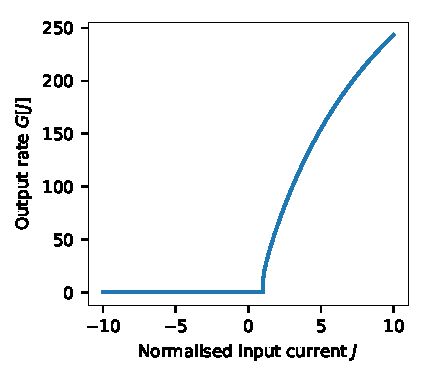
\includegraphics[width=0.7\textwidth]{media/nonlinearity_lif.pdf}%
	\end{columns}
\end{frame}

\begin{frame}
	\begin{columns}
		\column{0.8\textwidth}
		\begin{itemize}
			\item Does this work for all tuning curves?
			\vspace*{-0.3cm}			
			\begin{align*}
				a_i(x) &= G(\alpha_i x + J^\mathrm{bias}_i)			
			\end{align*}			
			\item<2-> a) increasing: Yes!
			\item<3-> b) decreasing: Yes! (just let $\alpha_i$ be negative)
			\begin{itemize}
			\item or, better yet, introduce $e_i$ which is either 1 or -1 and keep $\alpha_i$ to be always positive.  This keeps the two ideas (slope and increase/decreasing) separate. 
			\end{itemize}
			\vspace*{-0.3cm}
			\begin{align*}
				a_i(x) &= G(\alpha_i (e_i x) + J^\mathrm{bias}_i)			
			\end{align*}			
			\item<4-> c) preferred stimulus: Need some sort of similarity measure
			\begin{itemize}
				\item<4-> But it shouldn't be too complicated.  So far we've only needed to introduce multiplication and addition, which are both things we're pretty sure neurons can do, so let's avoid adding anything else if we don't have to.  Ideas?
			\end{itemize} 
			\vspace*{-0.3cm}		
			\begin{align*}
				a_i(x) &= G(\alpha_i sim(e_i, x) + J^\mathrm{bias}_i)			
			\end{align*}			
		\end{itemize}
		\column{0.2\textwidth}
		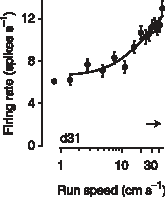
\includegraphics[scale=0.75]{media/saleem_et_al_tuning_curves_a.pdf} \\
		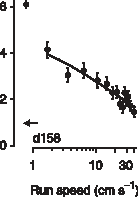
\includegraphics[scale=0.75]{media/saleem_et_al_tuning_curves_c.pdf} \\
		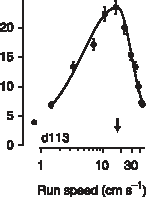
\includegraphics[scale=0.75]{media/saleem_et_al_tuning_curves_b.pdf}
	\end{columns}
\end{frame}

\begin{frame}{Encoders: Preferred Direction Vectors}
	\begin{itemize}
		\item The represented value $x$ doesn't have to be a scalar
		\item What if it's a vector?
		\item<2-> There's a simple similarity-like measure for vectors: the dot product
		\begin{align*}
			\langle \vec x, \vec y \rangle = \sum_{i = 0}^d x_i y_i = \cos(\angle(\vec x, \vec y)) \| \vec x\| \| \vec y\|
		\end{align*}					
		\begin{align*}
			a_i(\vec x) &= G(\alpha_i \langle \vec e_i, \vec x \rangle + J^\mathrm{bias}_i)			
		\end{align*}
		\item<2-> Constrain $e_i$ to be a unit vector
		\begin{itemize}
			\item Note that for scalar $x$, the only two unit vectors are +1 and -1
			\item So the increasing / decreasing scenario is a special case of this!
		\end{itemize}					
	\end{itemize}
\end{frame}

\begin{frame}{Preferred Directions in Higher Dimensions: Representing 2D Values}
	\begin{columns}[c]
		\column{0.5\textwidth}
		\centering
		\includegraphics<1->[height=5.75cm,trim=1cm 0cm 0cm 1cm,clip]{media/2d_encoder_tuning_curve.pdf}
		\column{0.5\textwidth}
		\centering
		\includegraphics<2->[height=5.75cm]{media/2d_encoder_tuning_curve_unit.pdf}	
	\end{columns}
\end{frame}


\begin{frame}{Decoding}
	\begin{itemize}
		\item Non-linear Encoding and Linear Decoding
		\begin{align*}
			\vec a_i &=
			G\big[\alpha_i \langle \vec x, \vec e_i \rangle + J^\mathrm{bias}_i\big] \,, && \text{Encoding} \\
			\hat{\vec x} &= \mat D \vec a && \text{Decoding}
		\end{align*}
		\item How do we find $\mat D$?
		\item<2-> Least-squares minimization
		\begin{align*}
			\arg\min_{\mat D} E = \frac{1}{|\mathbb{X}|} \int_{\mathbb{X}} \|\vec x - \hat{\vec x}\| \,\mathrm{d}\vec x = \frac{1}{|\mathbb{X}|} \int_{\mathbb{X}} \|\vec x - \mat D \vec a(\vec x)\| \,\mathrm{d}\vec x
		\end{align*}
	\end{itemize}
\end{frame}

\begin{frame}{Decoding via Least-squares Minimization}
	\begin{itemize}
		\item Find the minimum decoding error
	\begin{align*}
		\arg\min_{\mat D} E = \frac{1}{|\mathbb{X}|} \int_{\mathbb{X}} \|\vec x - \hat{\vec x}\| \,\mathrm{d}\vec x = \frac{1}{|\mathbb{X}|} \int_{\mathbb{X}} \|\vec x - \mat D \vec a(\vec x)\| \,\mathrm{d}\vec x
	\end{align*}
		\item Can't do that analytically (in general), so let's sample
	\begin{align*}
	\arg\min_{\mat D} E = \frac{1}{N} \sum_{i=0}^N \|\vec x_i - \mat D \vec a(\vec x_i)\| \,
	\end{align*}
\end{itemize}
	
\end{frame}

\begin{frame}{Decoding via Least-squares Minimization}
	\begin{itemize}
		\item Let's write this in matrix form, where $\mat A_{ik} = a_i(x_k)$ and $\vec X = (x_1, \ldots, x_N)$
		\item We want $\mat A^T \mat D^T = \mat X^T$
		\item So $\mat A \mat A^T \mat D^T = \mat A \mat X^T$
		\item $(\mat A \mat A^T)^{-1}\mat A \mat A^T \mat D^T = (\mat A \mat A^T)^{-1}\mat A \mat X^T$ 
		\item $\mat D^T = (\mat A \mat A^T)^{-1}\mat A \mat X^T$
		\item In Python, \texttt{D = np.linalg.lstsq(A.T, X.T, rcond=None)[0].T}
		\item (where \texttt{A} is a n x N array and \texttt{X} is a d x N array)
	\end{itemize}
\end{frame}

\begin{frame}{Decoding}
	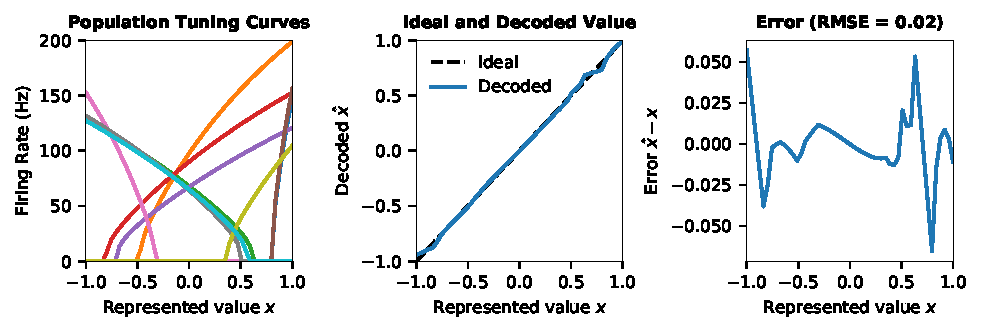
\includegraphics[width=\textwidth]{media/decoding_example_no_noise.pdf}
	\begin{columns}
		\column{0.20\textwidth}
		$\mat A$
		\column{0.20\textwidth}
		$\mat A^T \mat D^T$
		\column{0.20\textwidth}
		$\mat A^T \mat D^T - \mat X^T$
	\end{columns}
\end{frame}

\begin{frame}{Sources of Noise in Biological Neural Networks}
	\begin{columns}
		\column{0.5\textwidth}
		\begin{itemize}
			\item \textbf{Axonal jitter}\\
			Active axonal spike propagation
			\item \textbf{Vesicle release failure}\\
			10-30\% of pre-synaptic events cause post-synaptic current
			\item \textbf{Neurotransmitter per vesicle}\\
			Varying amounts of neurotransmitter\\
			\item \textbf{Ion channel noise}\\
			Ion-channels are \enquote{binary}, stochastic
			\item \textbf{Thermal noise}
			\item \textbf{Network effects}\\
			Simple, noise-free inhibitory/excitatory networks produce irregular spike trains
		\end{itemize}
		\column{0.5\textwidth}
			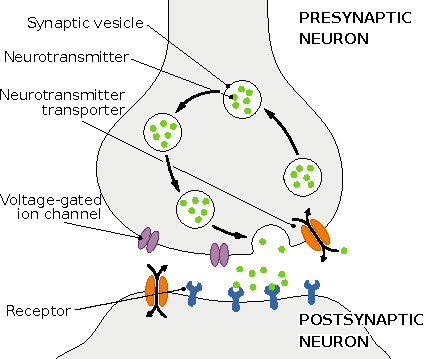
\includegraphics[width=\textwidth]{media/synapse_schematic.pdf}
			\begin{itemize}			
				\item<2-> \hl{How to model?} \only<3->{Gaussian noise}
			\end{itemize}
	\end{columns}
\end{frame}

\begin{frame}{NEF Principle 0: Noise}
\begin{mdframed}
	\textbf{NEF Principle 0 -- Noise}\\
	Biological neural systems are subject to significant amounts of noise from various sources. Any analysis of such systems must take the effects of noise into account.
\end{mdframed}
\end{frame}

\begin{frame}{Decoding Noisy $\mat A$ Without Taking Noise Into Account}
	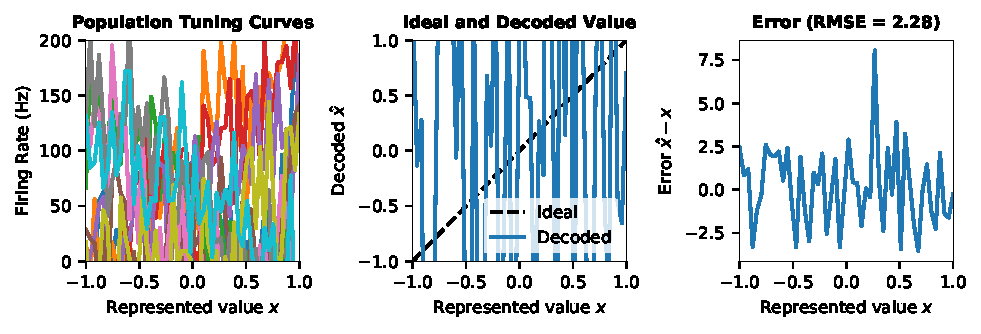
\includegraphics[width=\textwidth]{media/decoding_example_noise.pdf}
\end{frame}

\begin{frame}{Decoding Noisy $\mat A$ Accounting for Noise}
	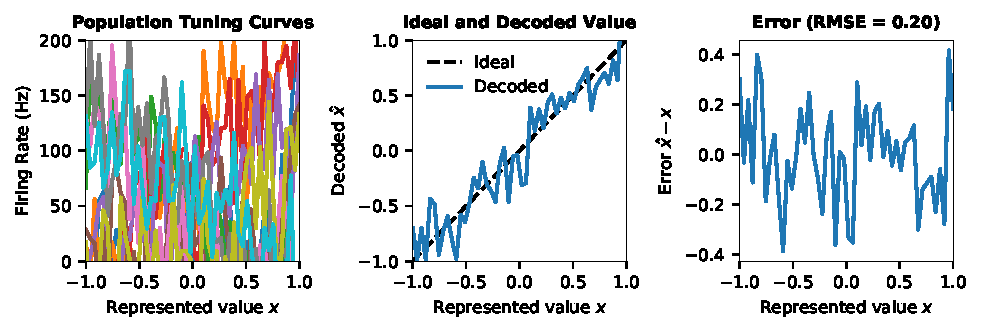
\includegraphics[width=\textwidth]{media/decoding_example_noise_accounted.pdf}
\end{frame}

\begin{frame}{Summary: Building a model of neural representation (Encoding)}
	\begin{columns}[c]
		\column{0.5\textwidth}
		\begin{block}{\hl{Encoding}}
		\begin{itemize}
			\setlength{\itemsep}{0.25cm}
			\item Select $d$, possible range $\vec x \in \mathbb{X}$, usually $\mathbb{X} = \big\{ \vec x \mid \| \vec x \| \leq r, \vec x \in \mathbb{R}^d \big\}$ ($r = 1$)
			\item Select number of neurons $n$
			\item Select tuning curves, maximum rates\\$\Rightarrow$ $\vec e_i$, $\alpha_i$, $J^\mathrm{bias}_i$\\[0.125cm]
			\begin{itemize}
				\setlength{\itemsep}{0.125cm}
				\item Sample $\vec e_i$ from unit-sphere
				\item Uniformly distribute $x$-intercept, maximum~rate
			\end{itemize}
			\item Encoding equation:\vspace{-0.25cm}
			$$a_i(\vec x) = G\big[ \alpha_i \langle \vec e_i, \vec x \rangle + J^\mathrm{bias}_i\big]$$
		\end{itemize}
		\end{block}
		\column{0.5\textwidth}
		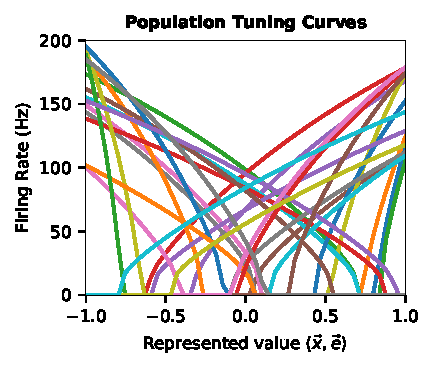
\includegraphics{media/tuning_curves.pdf}
	\end{columns}
\end{frame}

\begin{frame}{Summary: Building a model of neural representation (Decoding)}
	\begin{columns}
		\column{0.5\textwidth}
		\begin{block}{\hl{Decoding}}
		\begin{itemize}
			\setlength{\itemsep}{0.25cm}
			\item Uniformly sample $N$ samples from $\mathbb{X}$, $\mat X = \big( \vec x_1, \ldots, \vec x_N \big)$
			\item Compute $\mat A$, where $(\mat A)_{ik} = a_i(\vec x_k)$
			\item Decoder computation:\vspace{-0.25cm}
			$$\mat D^\T = \big( \mat A \mat A^\T + N \sigma^2 \mat I \big)^{-1} \mat A \mat X^\T$$
			\item Decoding equation:\vspace{-0.25cm}
			$$\hat{\mat X} = \mat D \mat A$$
		\end{itemize}
		\end{block}
		\column{0.5\textwidth}
		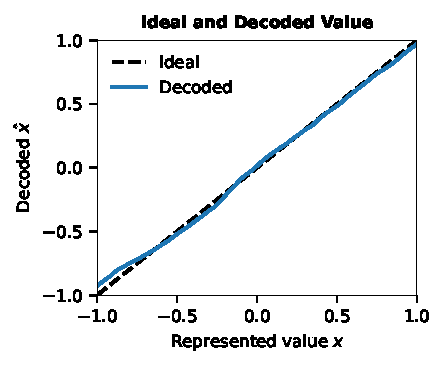
\includegraphics{media/decoding.pdf}
	\end{columns}
\end{frame}

\begin{frame}{Analysing Sources of Errors}
	\centering
	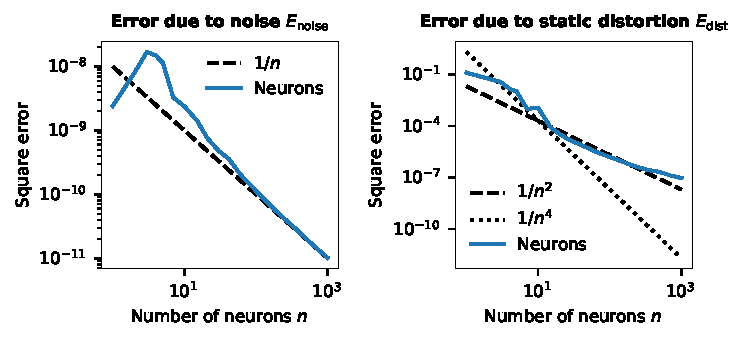
\includegraphics[width=0.75\textwidth]{media/error_experiment.pdf}
	\begin{align*}
		E &= \underbrace{\frac{1}2 \int_{-1}^1 \left(x - \sum_{i = 1}^n d_i a_i(x) \right)^2 \,\mathrm{d}x}_{E_\mathrm{dist}} + \underbrace{\frac{1}2 \sigma^2 \sum_{i = 1}^n d_i^2}_{E_\mathrm{noise}}
	\end{align*}
\end{frame}

\begin{frame}{Example: Horizontal Eye Position (1D)}
	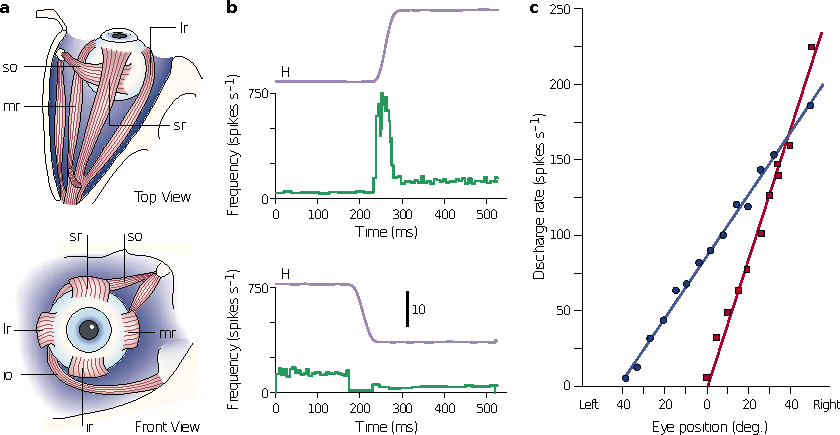
\includegraphics[width=\textwidth]{media/sparks_et_al_2002_brainstem_eye.pdf}
\end{frame}

\begin{frame}{Example: Horizontal Eye Position (1D) (cont.)}
	\begin{multicols}{2}
		\begin{itemize}
			\setlength{\itemsep}{0.5cm}
			\item \textbf{Step 1: System Description}
			\begin{itemize}
				\setlength{\itemsep}{0.5cm}
				\item What is being represented?
				\begin{itemize}
					\setlength{\itemsep}{0.25cm}
					\item $x$ is the horizontal eye position
				\end{itemize}
				\item What is the tuning curve shape?
				\begin{itemize}
					\setlength{\itemsep}{0.25cm}
					\item Linear, low $\tau_\mathrm{ref}$, high $\tau_\mathrm{RC}$
					\item $e_i \in \{1, -1\}$
					\item Firing rates up to \SI{300}{\per\second}
				\end{itemize}
			\end{itemize}
			\columnbreak
			\item \textbf{Step 2: Design Specification}
			\begin{itemize}
				\setlength{\itemsep}{0.25cm}
				\item Range of values
				\begin{itemize}
					\setlength{\itemsep}{0.25cm}
					\item $\mathbb{X} = [-60, 60]$
				\end{itemize}
				\item Amount of noise
				\begin{itemize}
					\setlength{\itemsep}{0.25cm}
					\item About $20\%$ of $\max(\mat A)$
				\end{itemize}
			\end{itemize}
			\item \textbf{Step 3: Implementation}
			\begin{itemize}
				\setlength{\itemsep}{0.25cm}
				\item Choose tuning curve parameters
				\item Compute decoders
			\end{itemize}
		\end{itemize}
	\end{multicols}
\end{frame}

\begin{frame}{Example: Arm Movements (2D)}
	\centering
	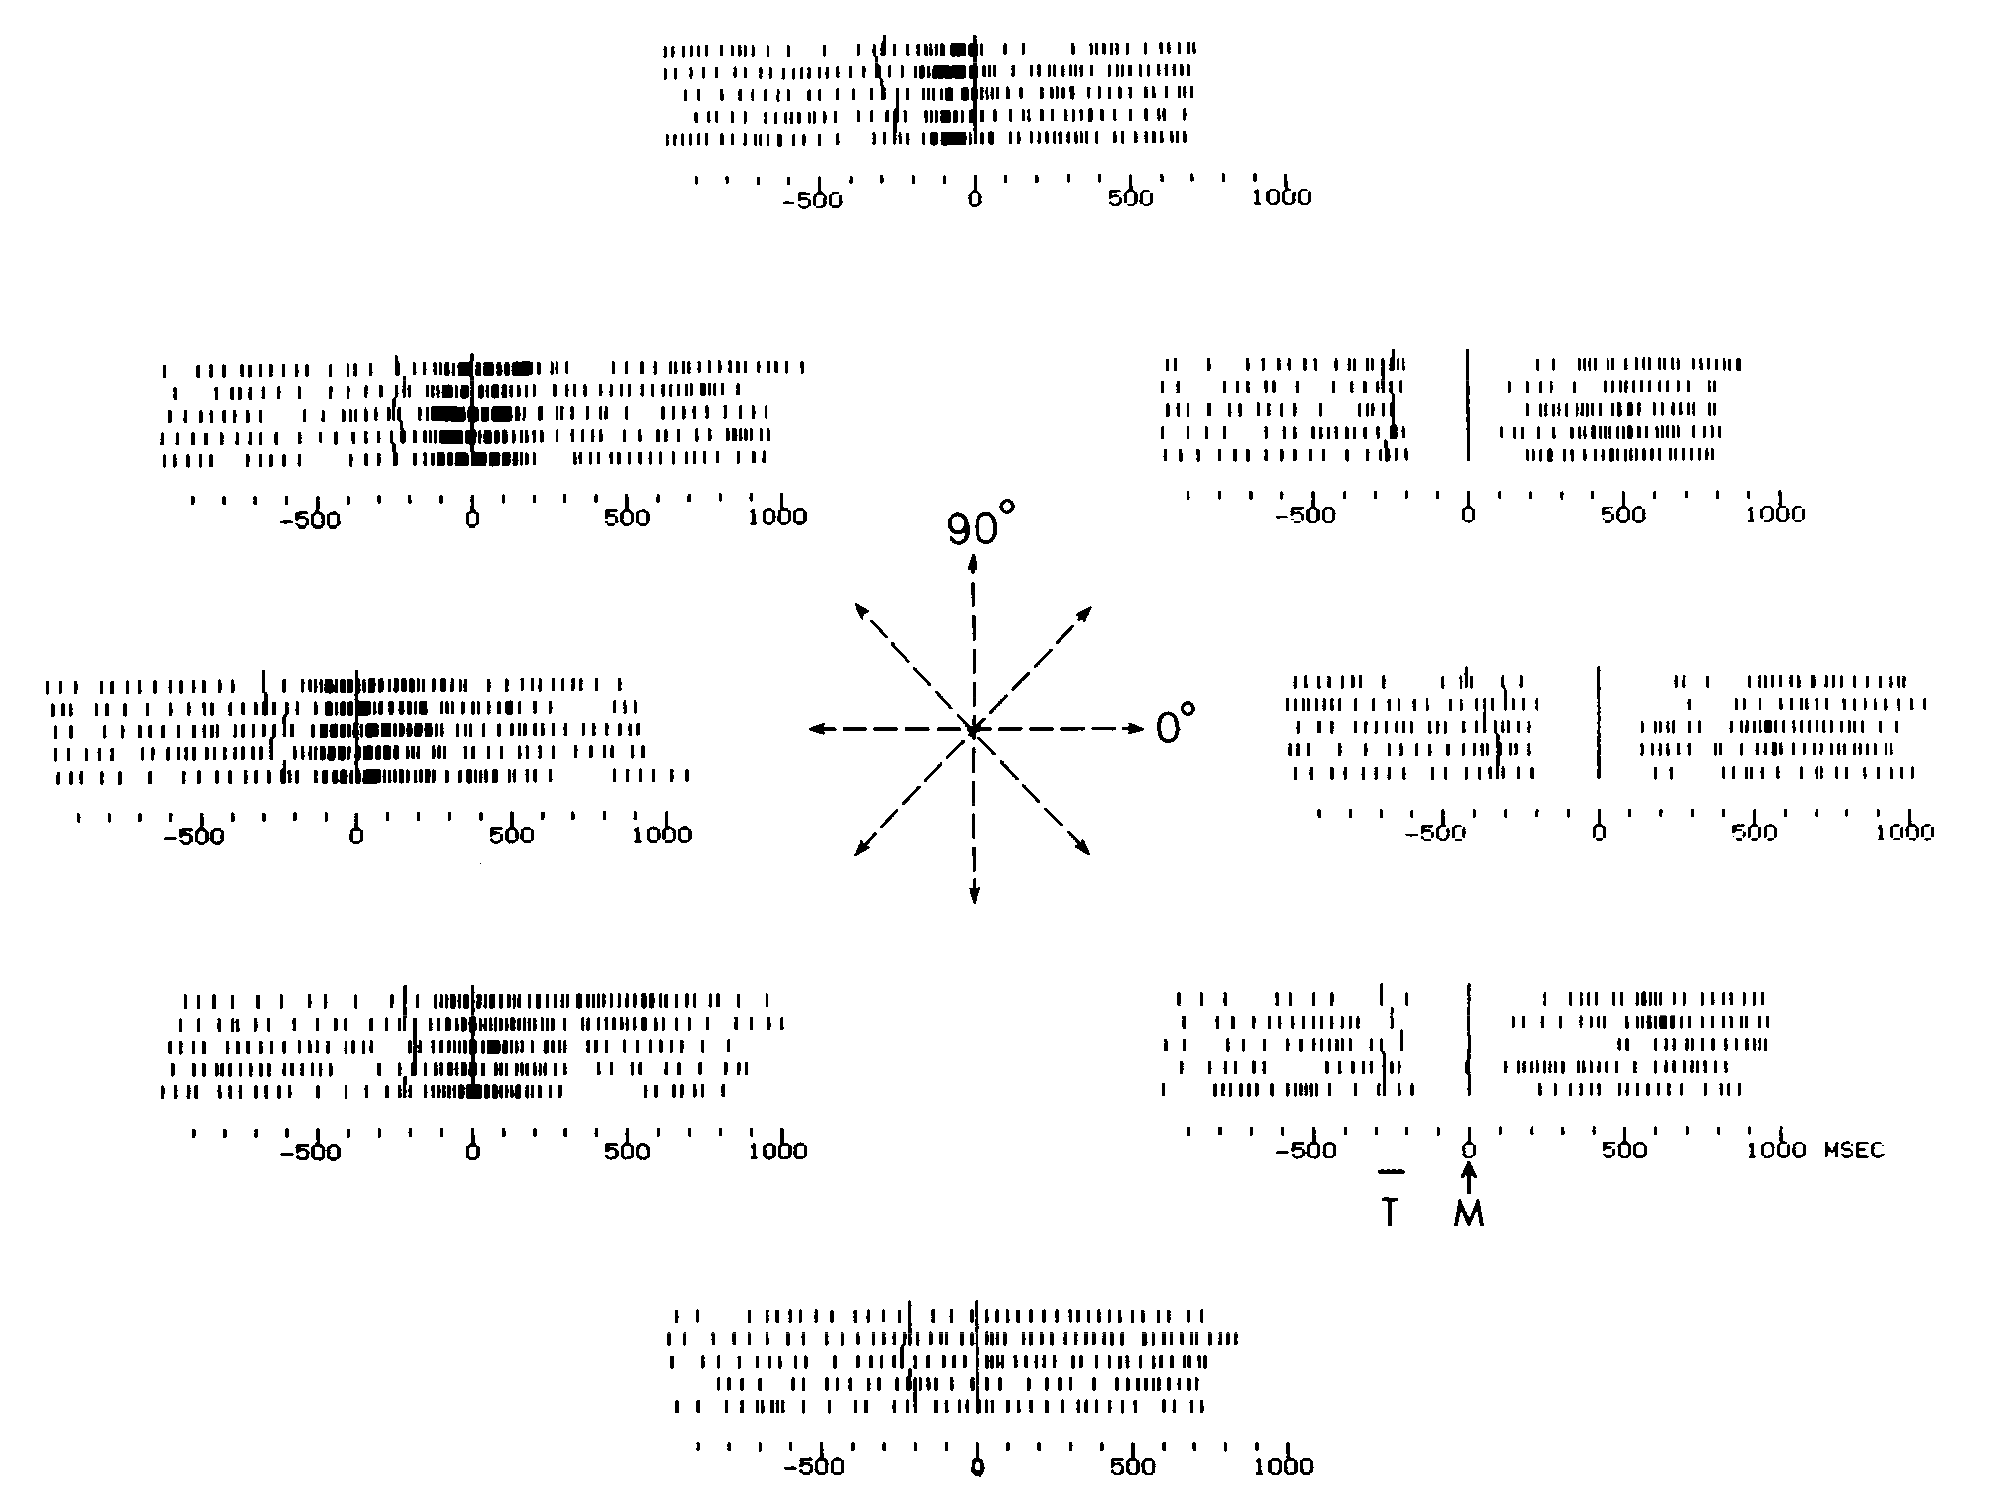
\includegraphics[width=0.5\textwidth]{media/georgopoulos_spike_raster.png}%
	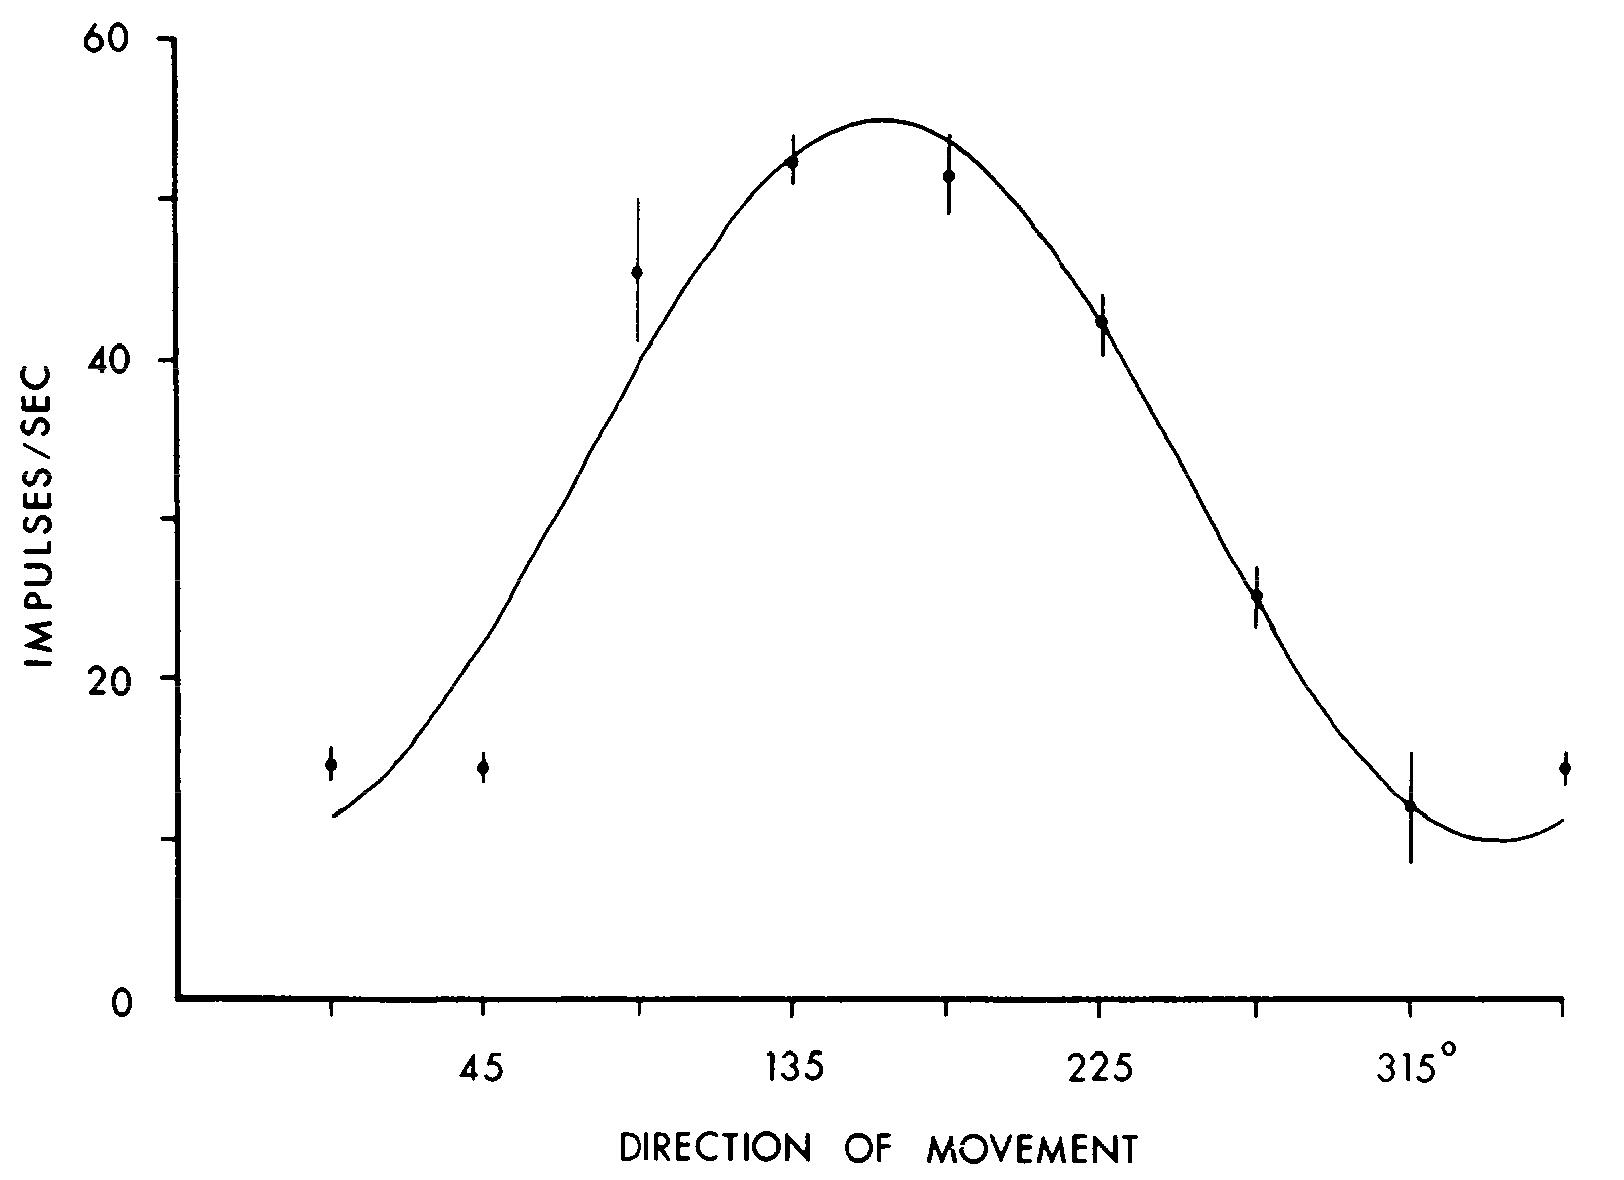
\includegraphics[width=0.5\textwidth]{media/georgopoulos_tuning.png}
\end{frame}

\begin{frame}{Example: Arm Movements (2D) (cont.)}
	\begin{columns}
		\column{0.4\textwidth}
		\centering
		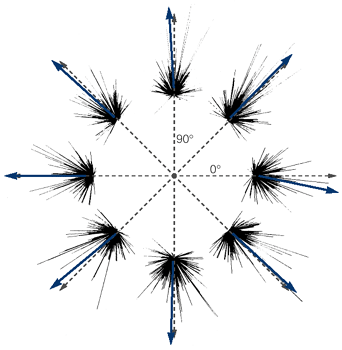
\includegraphics[width=0.9\textwidth]{media/georgopoulos_directions.png}%
		\column{0.6\textwidth}
		\begin{itemize}
			\setlength{\itemsep}{0.2cm}
			\item Experiment by Georgopoulos et~al., 1982
			\item Preferred arm movement directions $\vec e_i$
			\item \hl{Idea:} \emph{Population Vectors}, decode using
			\begin{align*}
				\hat{\vec x} &= \sum_{i=1}^n a_i(\vec x) \vec e_i = {\mat E} {\mat A}
			\end{align*}
			\item[\OPlus]<2-> Good direction estimate
			\item[\OMinus]<3-> Cannot reconstruct magnitude
			\item[]<4-> \hl{The NEF does not use population vectors!}
		\end{itemize}
	\end{columns}
\end{frame}

\begin{frame}{Example: Arm Movements (2D) (cont.)}
	\begin{multicols}{2}
		\begin{itemize}
			\setlength{\itemsep}{0.5cm}
			\item \textbf{Step 1: System Description}
			\begin{itemize}
				\setlength{\itemsep}{0.5cm}
				\item What is being represented?
				\begin{itemize}
					\setlength{\itemsep}{0.25cm}
					\item $\vec x$ the movement direction\\(or hand position)
				\end{itemize}
				\item What is the tuning curve shape?
				\begin{itemize}
					\setlength{\itemsep}{0.25cm}
					\item Bell-shaped
					\item Encoders are randomly distributed along the unit circle
					\item Firing rates up to \SI{60}{\per\second}
				\end{itemize}
			\end{itemize}
			\columnbreak
			\item \textbf{Step 2: Design Specification}
			\begin{itemize}
				\setlength{\itemsep}{0.25cm}
				\item Range of values
				\begin{itemize}
					\item $\mathbb{X} = \{\vec x \mid \|\vec x\| \leq r, \vec x \in \mathbb{R}^2 \}$
				\end{itemize}
				\item Amount of noise
				\begin{itemize}
					\setlength{\itemsep}{0.25cm}
					\item About $20\%$ of $\max(\mat A)$
				\end{itemize}
			\end{itemize}
			\item \textbf{Step 3: Implementation}
			\begin{itemize}
				\setlength{\itemsep}{0.25cm}
				\item Choose tuning curve parameters
				\item Compute decoders
			\end{itemize}
		\end{itemize}
	\end{multicols}
\end{frame}

\begin{frame}{Example: Higher Dimensional Representation}
	\begin{columns}[b]
		\column{0.5\textwidth}
		\centering
		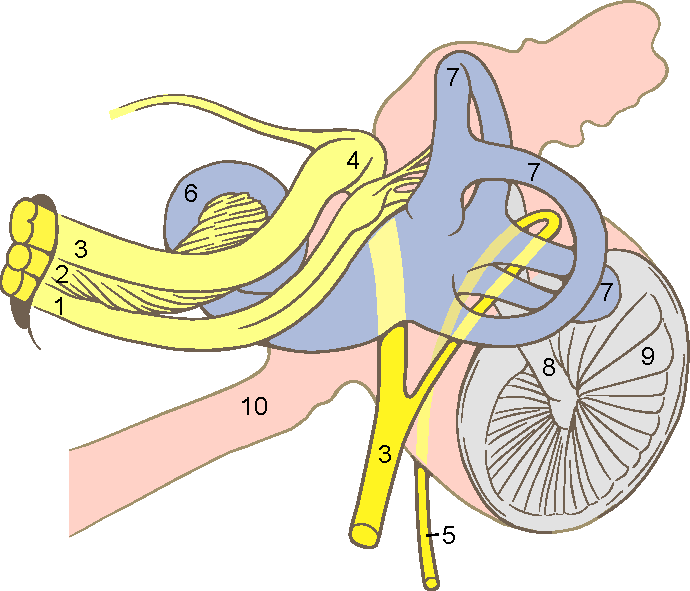
\includegraphics[width=0.8\textwidth]{media/ear_internal_anatomy_numbered.pdf}
		\column{0.5\textwidth}
		\centering
		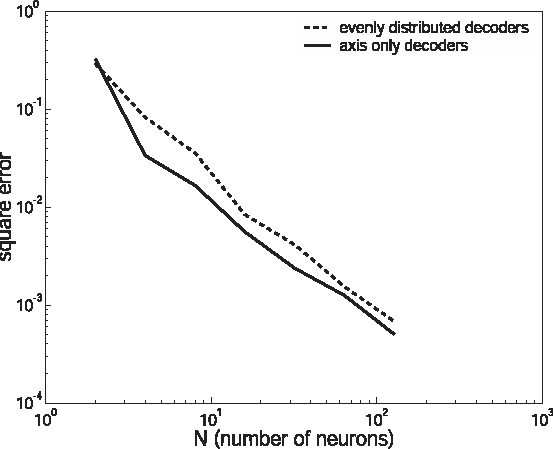
\includegraphics[width=0.8\textwidth]{media/eliasmith_et_al_2003_axis_aligned.pdf}%
	\end{columns}
	\begin{multicols}{2}
		\begin{itemize}
			\item Vestibular system senses head acceleration in 3D
			\item Axis aligned, must choose $\vec e_i \in$
			$\big\{ [1, 0, 0], [-1, 0, 0], \textellipsis, [0, 0, -1] \big\}$
			\columnbreak
			\item Same as three 1D populations
			\item Slightly lower precision
			\item<2-> \hl{Encoders affect accuracy}
		\end{itemize}
	\end{multicols}
\end{frame}

\backupbegin

\begin{frame}{Administration}
	\begin{itemize}
		\setlength{\itemsep}{0.75cm}
		\item \hl{Assignment 1 has been released.}\\[0.25cm]
		The due date is October 4, 2021.
	\end{itemize}
\end{frame}

\begin{frame}[noframenumbering]{Image sources}
	\small
	\textbf{Title slide}\\\enquote{The Ultimate painting.}\\Author: Clark Richert.\\From \href{https://commons.wikimedia.org/wiki/File:\%22The_Ultimate_painting\%22.jpg}{Wikimedia}.
\end{frame}


\backupend

\end{document}
